\section{Q4. Demonstration cases}
%Does the report show that the model checker can test some properties on a demonstration case? Which parts of the explanation are good? Which parts could be improved and how?

To demonstrate the model checker, we try model checking two different transition systems with model checks.\\

\subsection{Case: Tower of Hanoi}
The first transition system we model check, is the Tower of Hanoi with 3 discs and 3 rods. Defining the transition system requires the following lines of code.
\begin{lstlisting}
ts.add(1, true, new String[]{"AAA"}, new int[]{2, 3});
ts.add(2, false, new String[]{"BAA"}, new int[]{1, 3, 4});
ts.add(3, false, new String[]{"CAA"}, new int[]{1, 2, 5});
\end{lstlisting}
\vspace{-2mm}
\hspace{0.4\linewidth} \textbf{$\vdots$ }
\vspace{-2mm}
\begin{lstlisting}
ts.add(26, false, new String[]{"BCC"}, new int[]{19, 25, 27});
ts.add(27, false, new String[]{"CCC"}, new int[]{19, 26});
\end{lstlisting}

The states with atomic propositions are seen in figure \ref{fig:toh} from \textit{FMchap5} in the course material.

\begin{figure}[H]
    \centering
    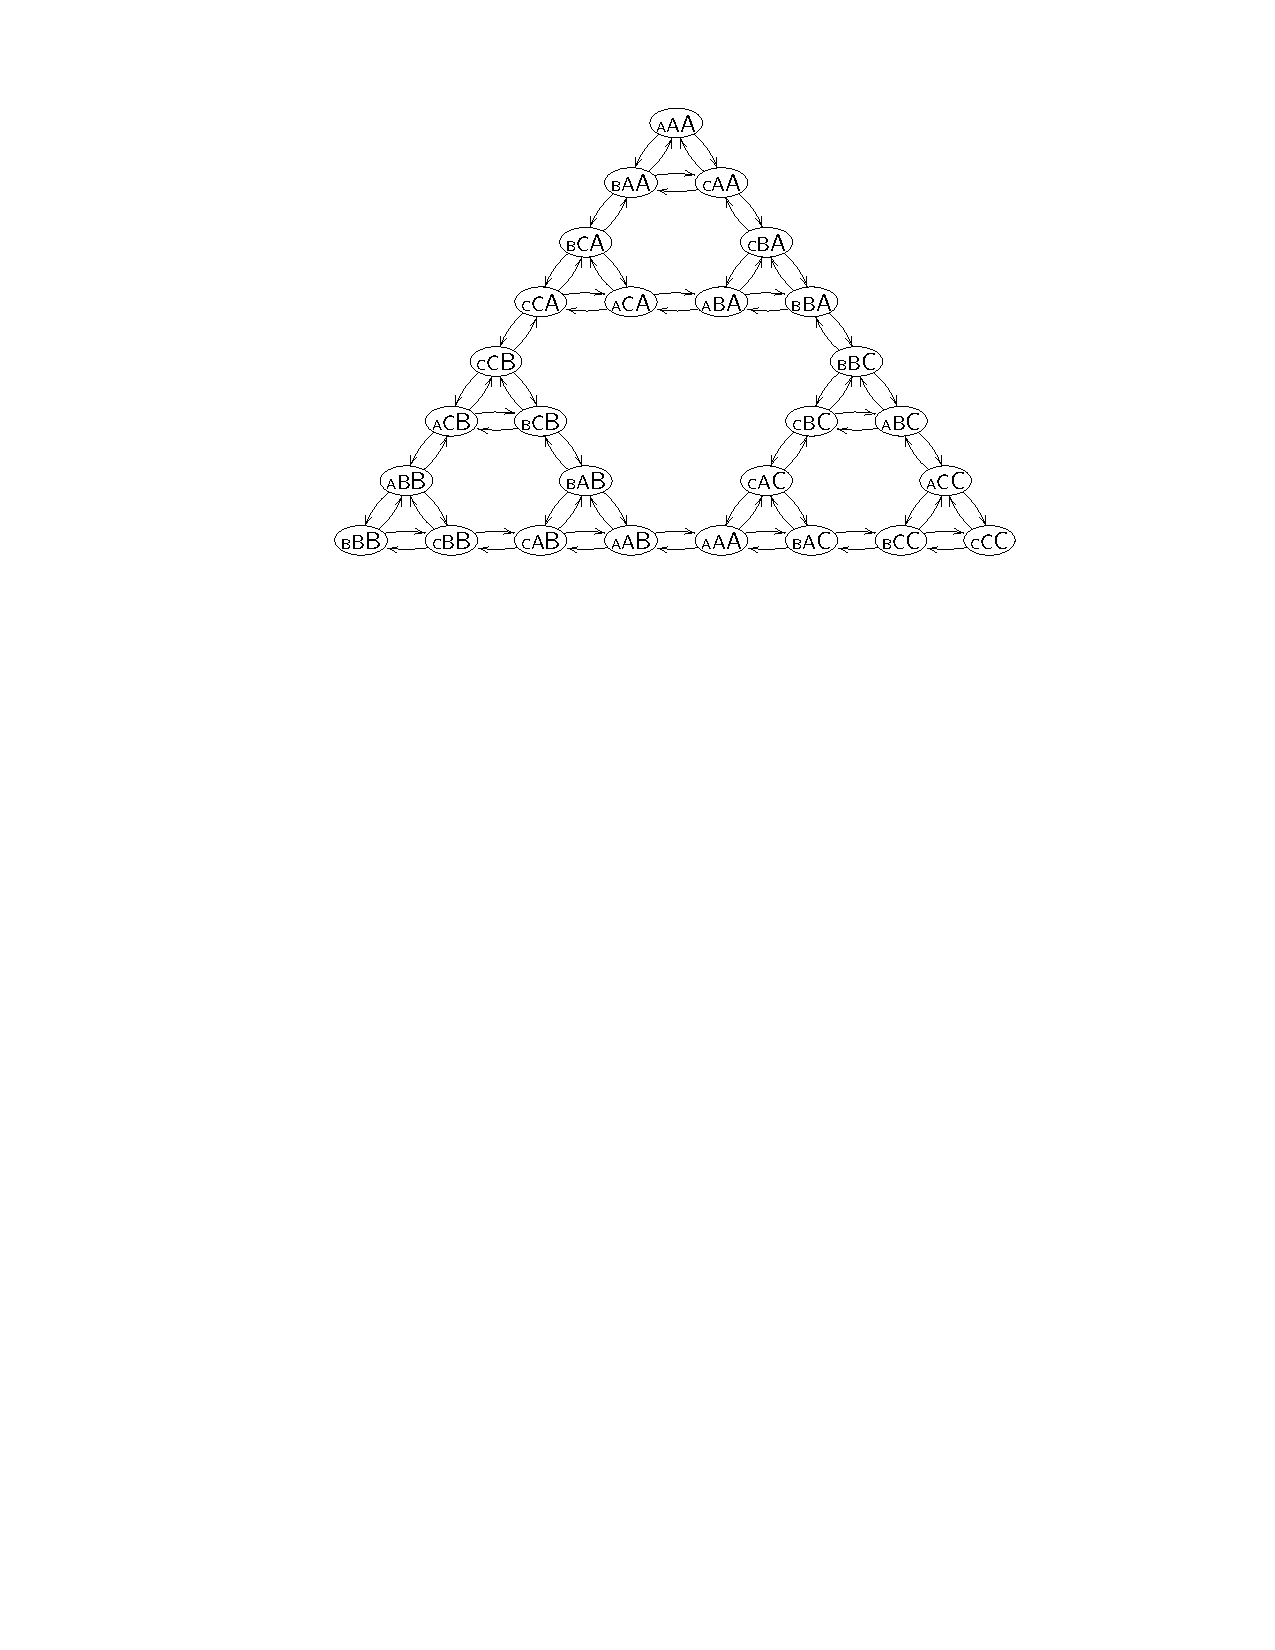
\includegraphics[width=0.6\textwidth]{fig/TowerOfHanoi.pdf}
    \caption{Tower of Hanoi for 3 discs and 3 rods. From \textit{FMchap5} in the course material. }
    \label{fig:toh}
\end{figure}

Since there exist at least one path from a state to any other state, a valid test is to check which states models $\models \exists \lozenge \; CCC$. The expected output would be all 27 states of the transition system. The actual output from the model checking is seen in figure \ref{fig:tohEFCCC}.\\

\begin{figure}[H]
    \centering
    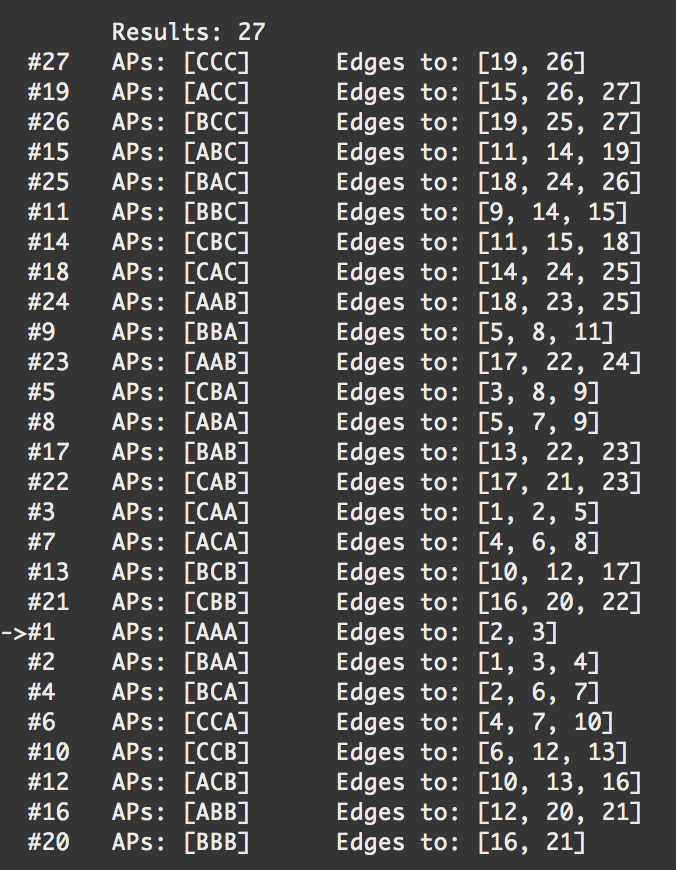
\includegraphics[width=0.5\textwidth]{fig/tohEFCCC.png}
    \caption{All states which models $\models \exists \lozenge \; CCC$ in Tower of Hanoi.}
    \label{fig:tohEFCCC}
\end{figure}

As seen in figure \ref{fig:tohEFCCC}, it is indeed all 27 states which satisfy the formula in the model checking. The order of the output is because it utilises back propagation to minimize computation time, see section \ref{sec:ctlEF}. \\

Alternatively since all states has unique atomic propositions, no state should model $\models \exists \square \; CCC$ (this is true for any atomic proposition, not just $CCC$). The actual output from the model checker is seen in figure \ref{fig:tohEGCCC}

\begin{figure}[H]
    \centering
    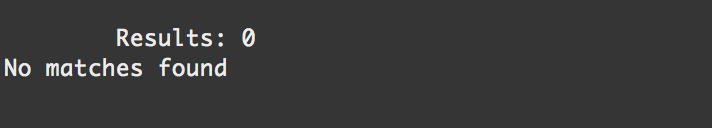
\includegraphics[width=0.5\textwidth]{fig/tohEGCCC.png}
    \caption{All states which models $\models \exists \square \; CCC$ in Tower of Hanoi.}
    \label{fig:tohEGCCC}
\end{figure}

As seen in figure \ref{fig:tohEGCCC} it is indeed true that no states model $\models \exists \square \; CCC$.

\subsection{Case 2: Restricted areas}
To check that the model checker also behaves as expected when the transition system has restricted areas, we test the transition system given in the assignment as seen in figure \ref{fig:restrictedsystem}.

\begin{figure}[H]
    \centering
    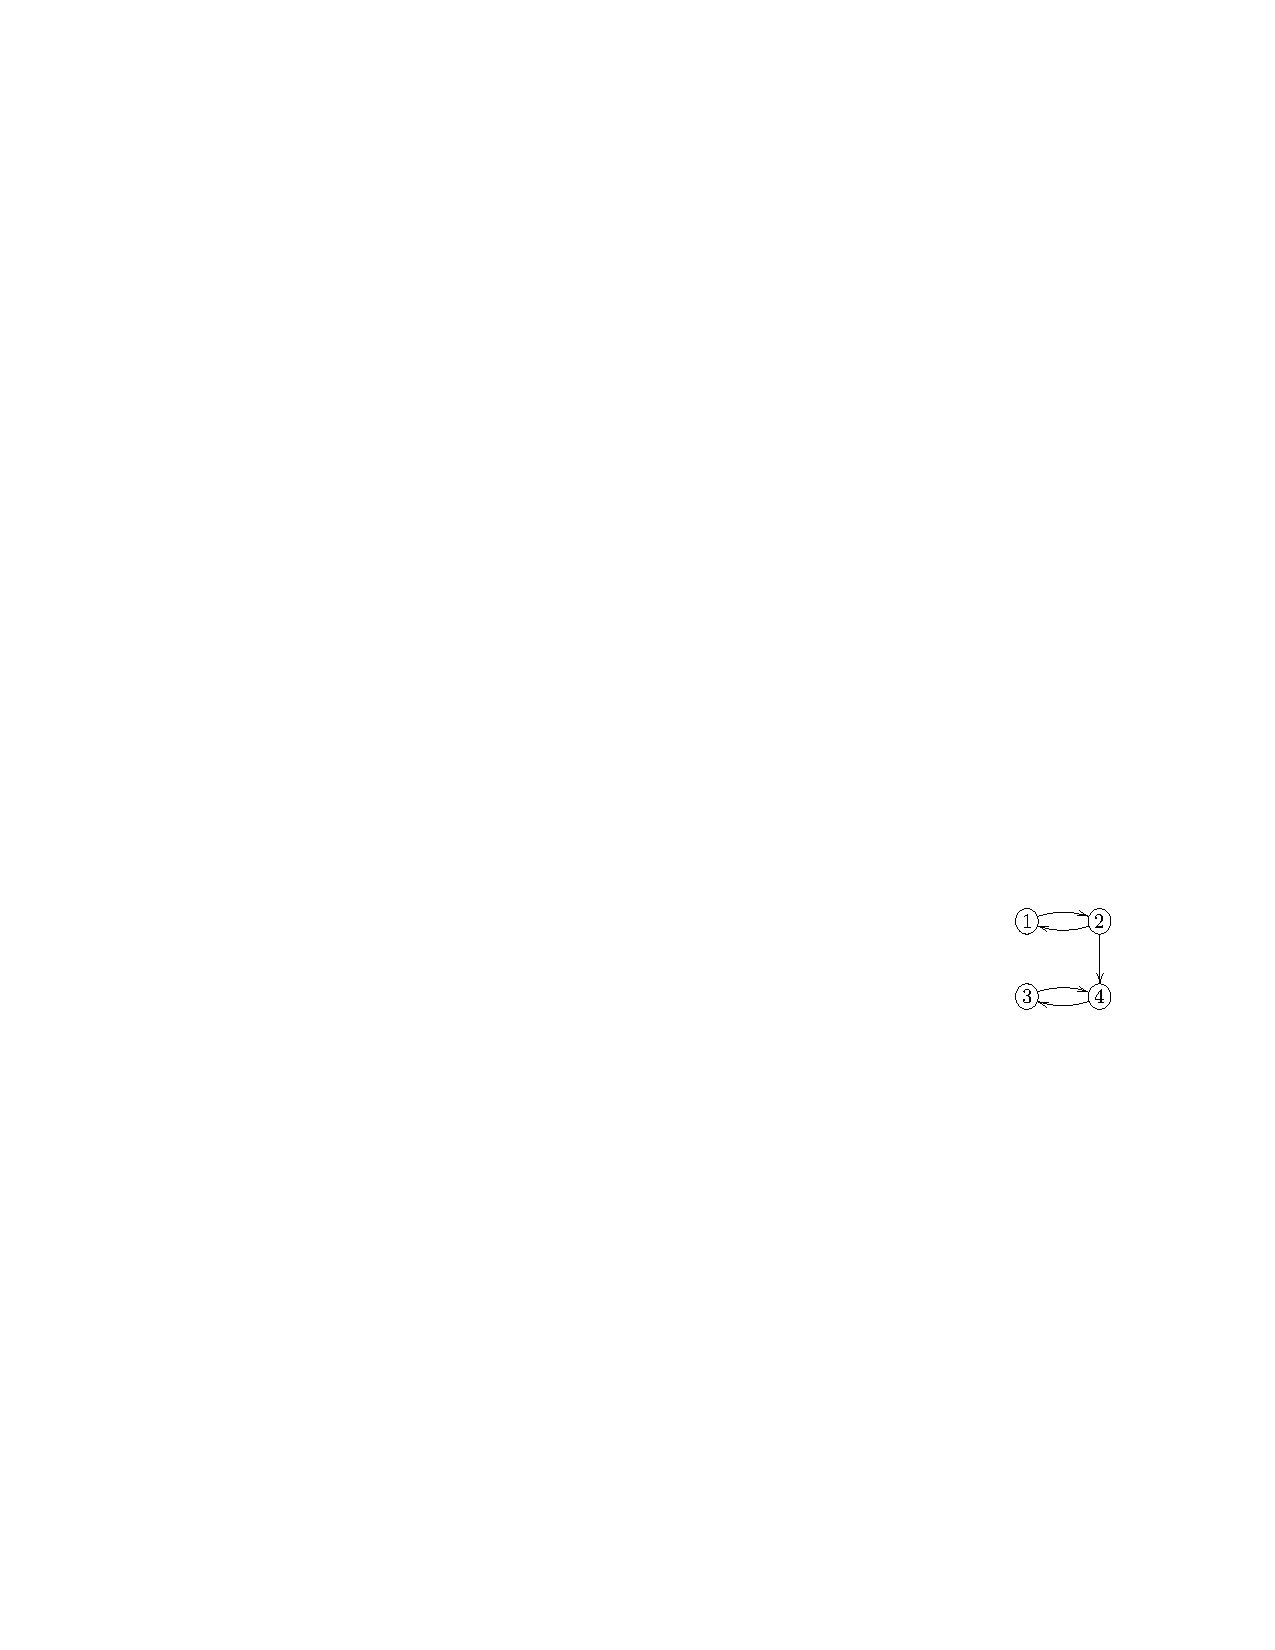
\includegraphics[width=0.15\textwidth]{fig/restrictedsystem.pdf}
    \caption{Example of a transition system with restricted areas. The system exists of the states \{1, 2, 3, 4\} with the respective atomic propositions \{v, v, c, c\}.}
    \label{fig:restrictedsystem}
\end{figure}

Defining the transition requires the following lines of code.
\begin{lstlisting}
ts.add(1, true, new String[]{"v"}, new int[]{2});
ts.add(2, false, new String[]{"v"}, new int[]{1, 4});
ts.add(3, false, new String[]{"c"}, new int[]{4});
ts.add(4, false, new String[]{"c"}, new int[]{3});
\end{lstlisting}

Since it is not possible to go from states 3 and 4 to states 1 or 2, only states 1 and 2 should model $\models \exists \lozenge \; v$. The actual output is seen in figure \ref{fig:rsEFv}

\begin{figure}[H]
    \centering
    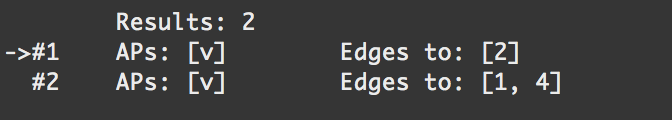
\includegraphics[width=0.5\textwidth]{fig/rsEFv.png}
    \caption{All states which models $\models \exists \lozenge \; v$ in the restricted system.}
    \label{fig:rsEFv}
\end{figure}

As seen in figure \ref{fig:rsEFv} the model checker returns the expected set of states.\\

This system also gives the opportunity to check if any states model $\models \forall \square \; c$ and if any states model $\models \exists \square \; v$. We expect that only states 3 and 4 satisfy the first formulae and only states 1 and 2 satisfy the second formulae. The output is seen in figure \ref{fig:rsAGcANDrsEGv}.

\begin{figure}[H]
    \begin{subfigure}{0.495\textwidth}
         \centering
        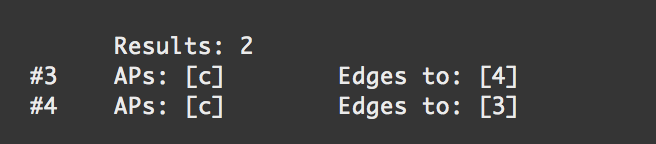
\includegraphics[width=0.9\linewidth, height=1.5cm]{fig/rsAGc.png} 
        \caption{All states which models $\models \forall \square \; c$.}
        \label{fig:rsAGc}
        \end{subfigure}
    \begin{subfigure}{0.495\textwidth}
         \centering
        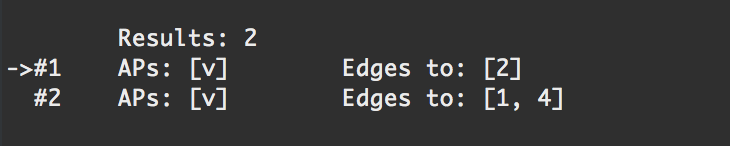
\includegraphics[width=0.9\linewidth, height=1.5cm]{fig/rsEGv.png}
        \caption{All states which models $\models \exists \square \; v$.}
        \label{fig:rsEGv}
    \end{subfigure}
     \caption{All states which models $\models \forall \square \; c$ or $\models \exists \square \; v$ in the restricted system.}
    \label{fig:rsAGcANDrsEGv}
\end{figure}

The model checker does indeed return the expected states.


